\subsection*{Ridge Regression}

Now that we have looked at performing the basis completeness extrapolations with traditional methods, we can develop a machine learning-based approach. A good machine learning algorithm will have a small number of hyperparameters to tune and give reproducible and accurate results for the extrapolation. Ridge regression only has one hyperparameter and a closed-form solution for its optimized weights. Therefore, it will always train the same way when given the same training data, making it a much more attractive alternative than neural networks, with their many hyperparameters and unrepeatable results.

The ridge regression algorithm contains one hyperparameter, $\alpha$, which is the strength of the regularization. Since this is a hyperparameter, the user must set its value before training the ridge regression algorithm. However, its value can significantly impact the results of the ridge regression. For example, figure \ref{fig:vary_alpha} shows the results of using the SRE algorithm with ridge regression and various $\alpha$ values to predict the converged $\Delta E_{CC}$ energies of the HEG with $r_s$ = 0.5.

\begin{figure}
    \centering
    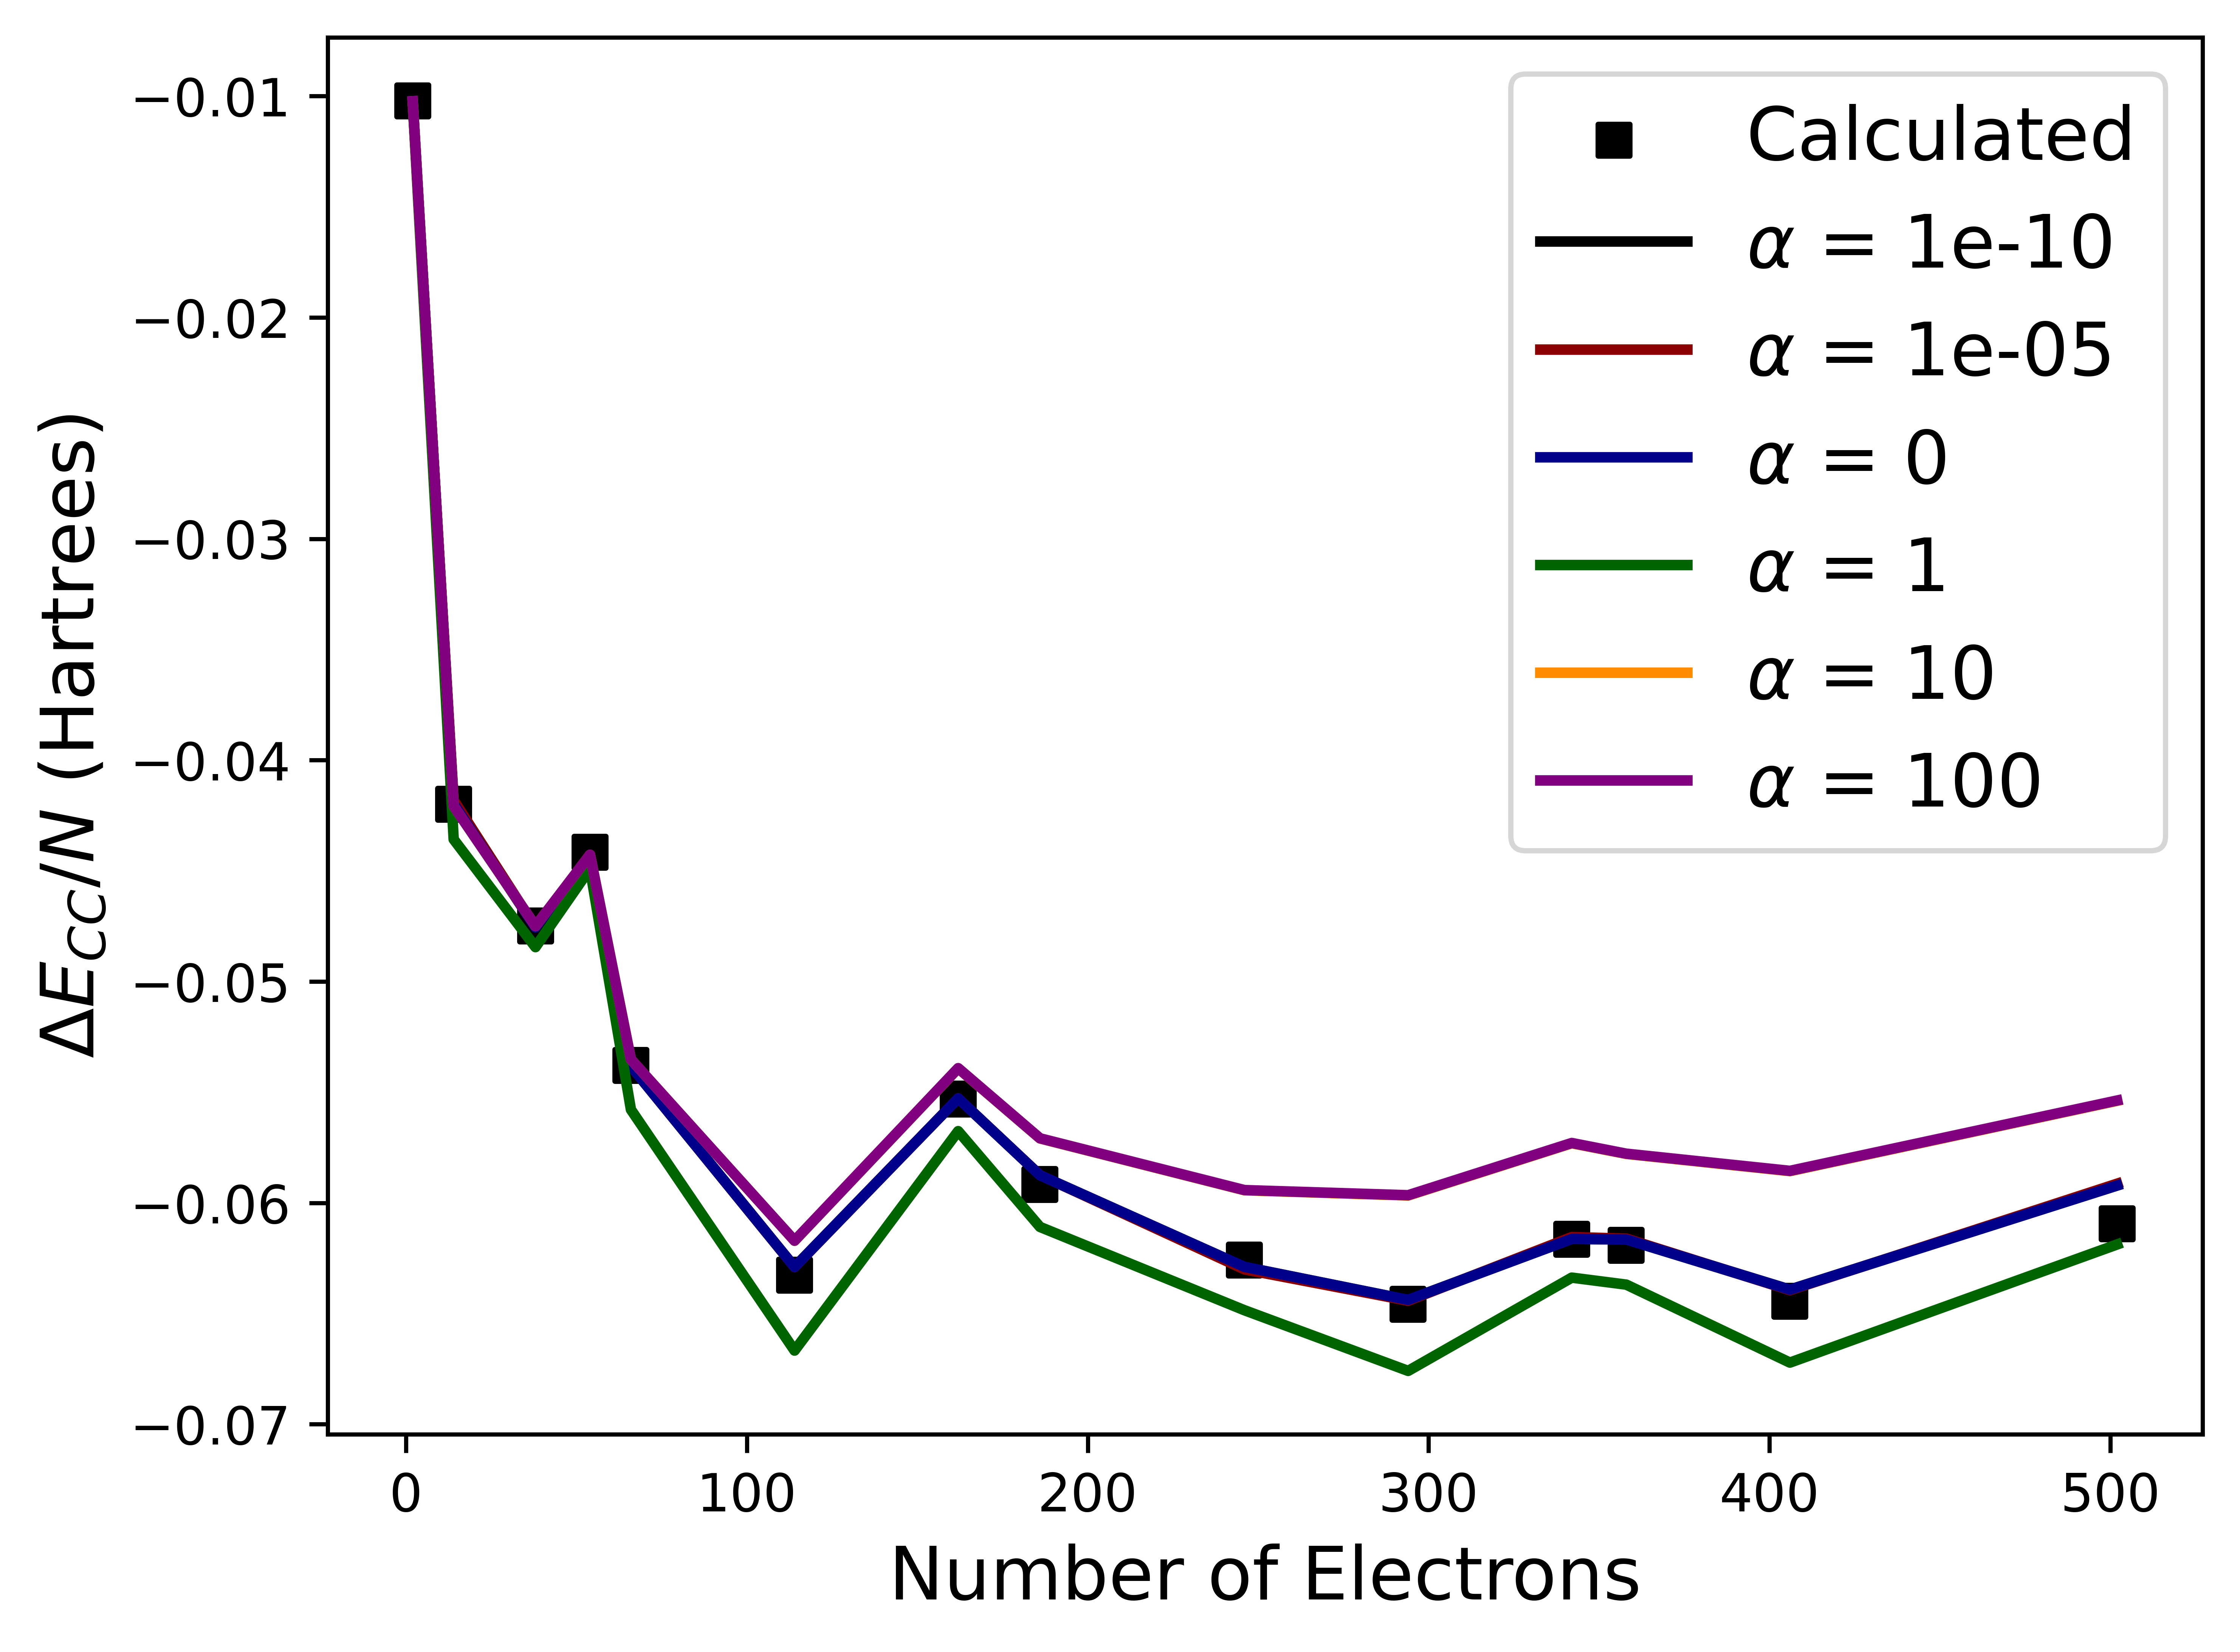
\includegraphics[scale=0.75]{Images/Chapter7/ElectronGas/vary_alpha.png}
    \caption{This figure shows the extrapolations' dependence on the hyperparameter $\alpha$. The results of performing an SRE analysis on the HEG with $r_s$ = 0.5 and at various numbers of electrons. The machine learning algorithm used for the SRE algorithm is ridge regression.}
    \label{fig:vary_alpha}
\end{figure}

For Fig. \ref{fig:vary_alpha}, the training data was chosen to be between 5 and 20 open shells (inclusive) or 2 $\leq$ M $\leq$ 2,090 (exact values of M depend on N). The sequence length for the SRE algorithm was set to 3, and the data set was extrapolated until there were 50 total points and the convergence was confirmed. The value of $\Delta E_{CC}$ we get from this process is considered converged. Therefore we will compare it to converged calculations of the HEG at M = 6,142, where the correlation energy convergence has converged. In Fig. \ref{fig:vary_alpha} $\Delta E_{CC, 6142}$ are plotted with scattered square points. These are considered to be the "true" or most accurate results. The solid lines show the results of performing the SRE algorithm to converge the correlation energy with respect to the number of single-particle states using the SRE algorithm with a variety of values for the hyperparameter $\alpha$.   Note that several of the values of $\alpha$ produce essentially equivalent results, so there are not six distinct lines. For $\alpha$ = 1x10$^{-10}$ and 1x10$^{-5}$ (which provide nearly identical results), the results are very close to the fully calculated converged correlation energies, with the average percent error overall numbers of electrons of 0.49$\%$. However, on the other hand, $\alpha$ = 1 and $\alpha$ = 100 provide results that visually appear to be suitable matches for the expected pattern in the data but do not match the converged calculations. However, if the fully converged calculations were not available for comparison, these could be considered reasonable predictions. For $\alpha$ = 1, the average percent error overall numbers of electrons is 3.09$\%$, and for $\alpha$ = 100, the average percent error is 3.87$\%$. Not shown in Fig. \ref{fig:vary_alpha} are the predictions for $\alpha$ = 1x10$^{-2}$ because the average percent error for the SRE algorithm's predictions and the actual data for this $\alpha$ value is 3.45x10$^{6}$$\%$. While this produces an undeniably incorrect result even if the actual data was not available for comparison, this shows the variation that can happen with the SRE predictions as $\alpha$ varies, and $\alpha$ values both larger and smaller than 1x10$^{-2}$ provide reasonable predictions, but $\alpha$ = 1x10$^{-2}$ provides predictions that do not converge.

A hyperparameter is typically set through a process known as hyperparameter tuning. In hyperparameter tuning, many different values are tested for the hyperparameters to find the best ones. First, the algorithm is defined using a given set of hyperparameters and trained using the training data; then, its accuracy is tested using a validation data set. The validation data set can be a subset of the training data, the test data, or a new data set altogether. This define-train-test cycle is repeated with many combinations of hyperparameters, and the hyperparameters that produce the lowest error on the validation data set are kept for future use.

For the HEG, we have data at five different values of $r_s$, so it was decided to choose one value of $r_s$ for hyperparameter tuning. Therefore, for the chosen value of $r_s$, not only does the SRE training data need to be generated, but the converged correlations energies at M = 6,142 also need to be generated will be a time-consuming process. When performing the hyperparameter tuning process on $\alpha$, 1,000 different values were tested, evenly spaced on a log scale between 1x10$^{-10}$ and 100 (inclusive). For each value, a ridge regression algorithm was defined with that value for $\alpha$. The ridge regression algorithm was used for an SRE analysis using the same training process described above. The predicted values for $\Delta E_{CC}$ were then compared to the fully converged calculations. The value for $\alpha$ that produced the lowest average percent error overall numbers of electrons was kept. This process was performed independently with all five different $r_s$ data sets to see how the results compare. 

When the hyperparameter tuning is performed using the data sets 0.1 $\leq$ $r_s$ $\leq$ 0.75, the optimal alpha value found was 1x10$^{-10}$. However, the hyperparameter tuning is performed on the data set at $r_s$ = 0.05, and the optimal alpha value was found to be 4.27x10$^{-4}$. When $\alpha$ = 1x10$^{-10}$ the average percent error for all $r_s$ values was 0.45$\%$, which is quite good and is a very acceptable error on the actual data for a prediction made with unconverted data. However, when $\alpha$ = 4.27x1-$^{-3}$ the average percent error for all $r_s$ values is 7.5x10$^{11}$$\%$, because some of the predictions do not converge.  When analyzing the results, this would be a wrong prediction, but as seen in Fig. \ref{fig:vary_alpha}, values of $\alpha$ could be chosen that provide seemingly good but incorrect answers. Moving forward with the ridge regression analysis, we will use $\alpha$ = 1x10$^{-10}$.

\begin{figure}
    \centering
    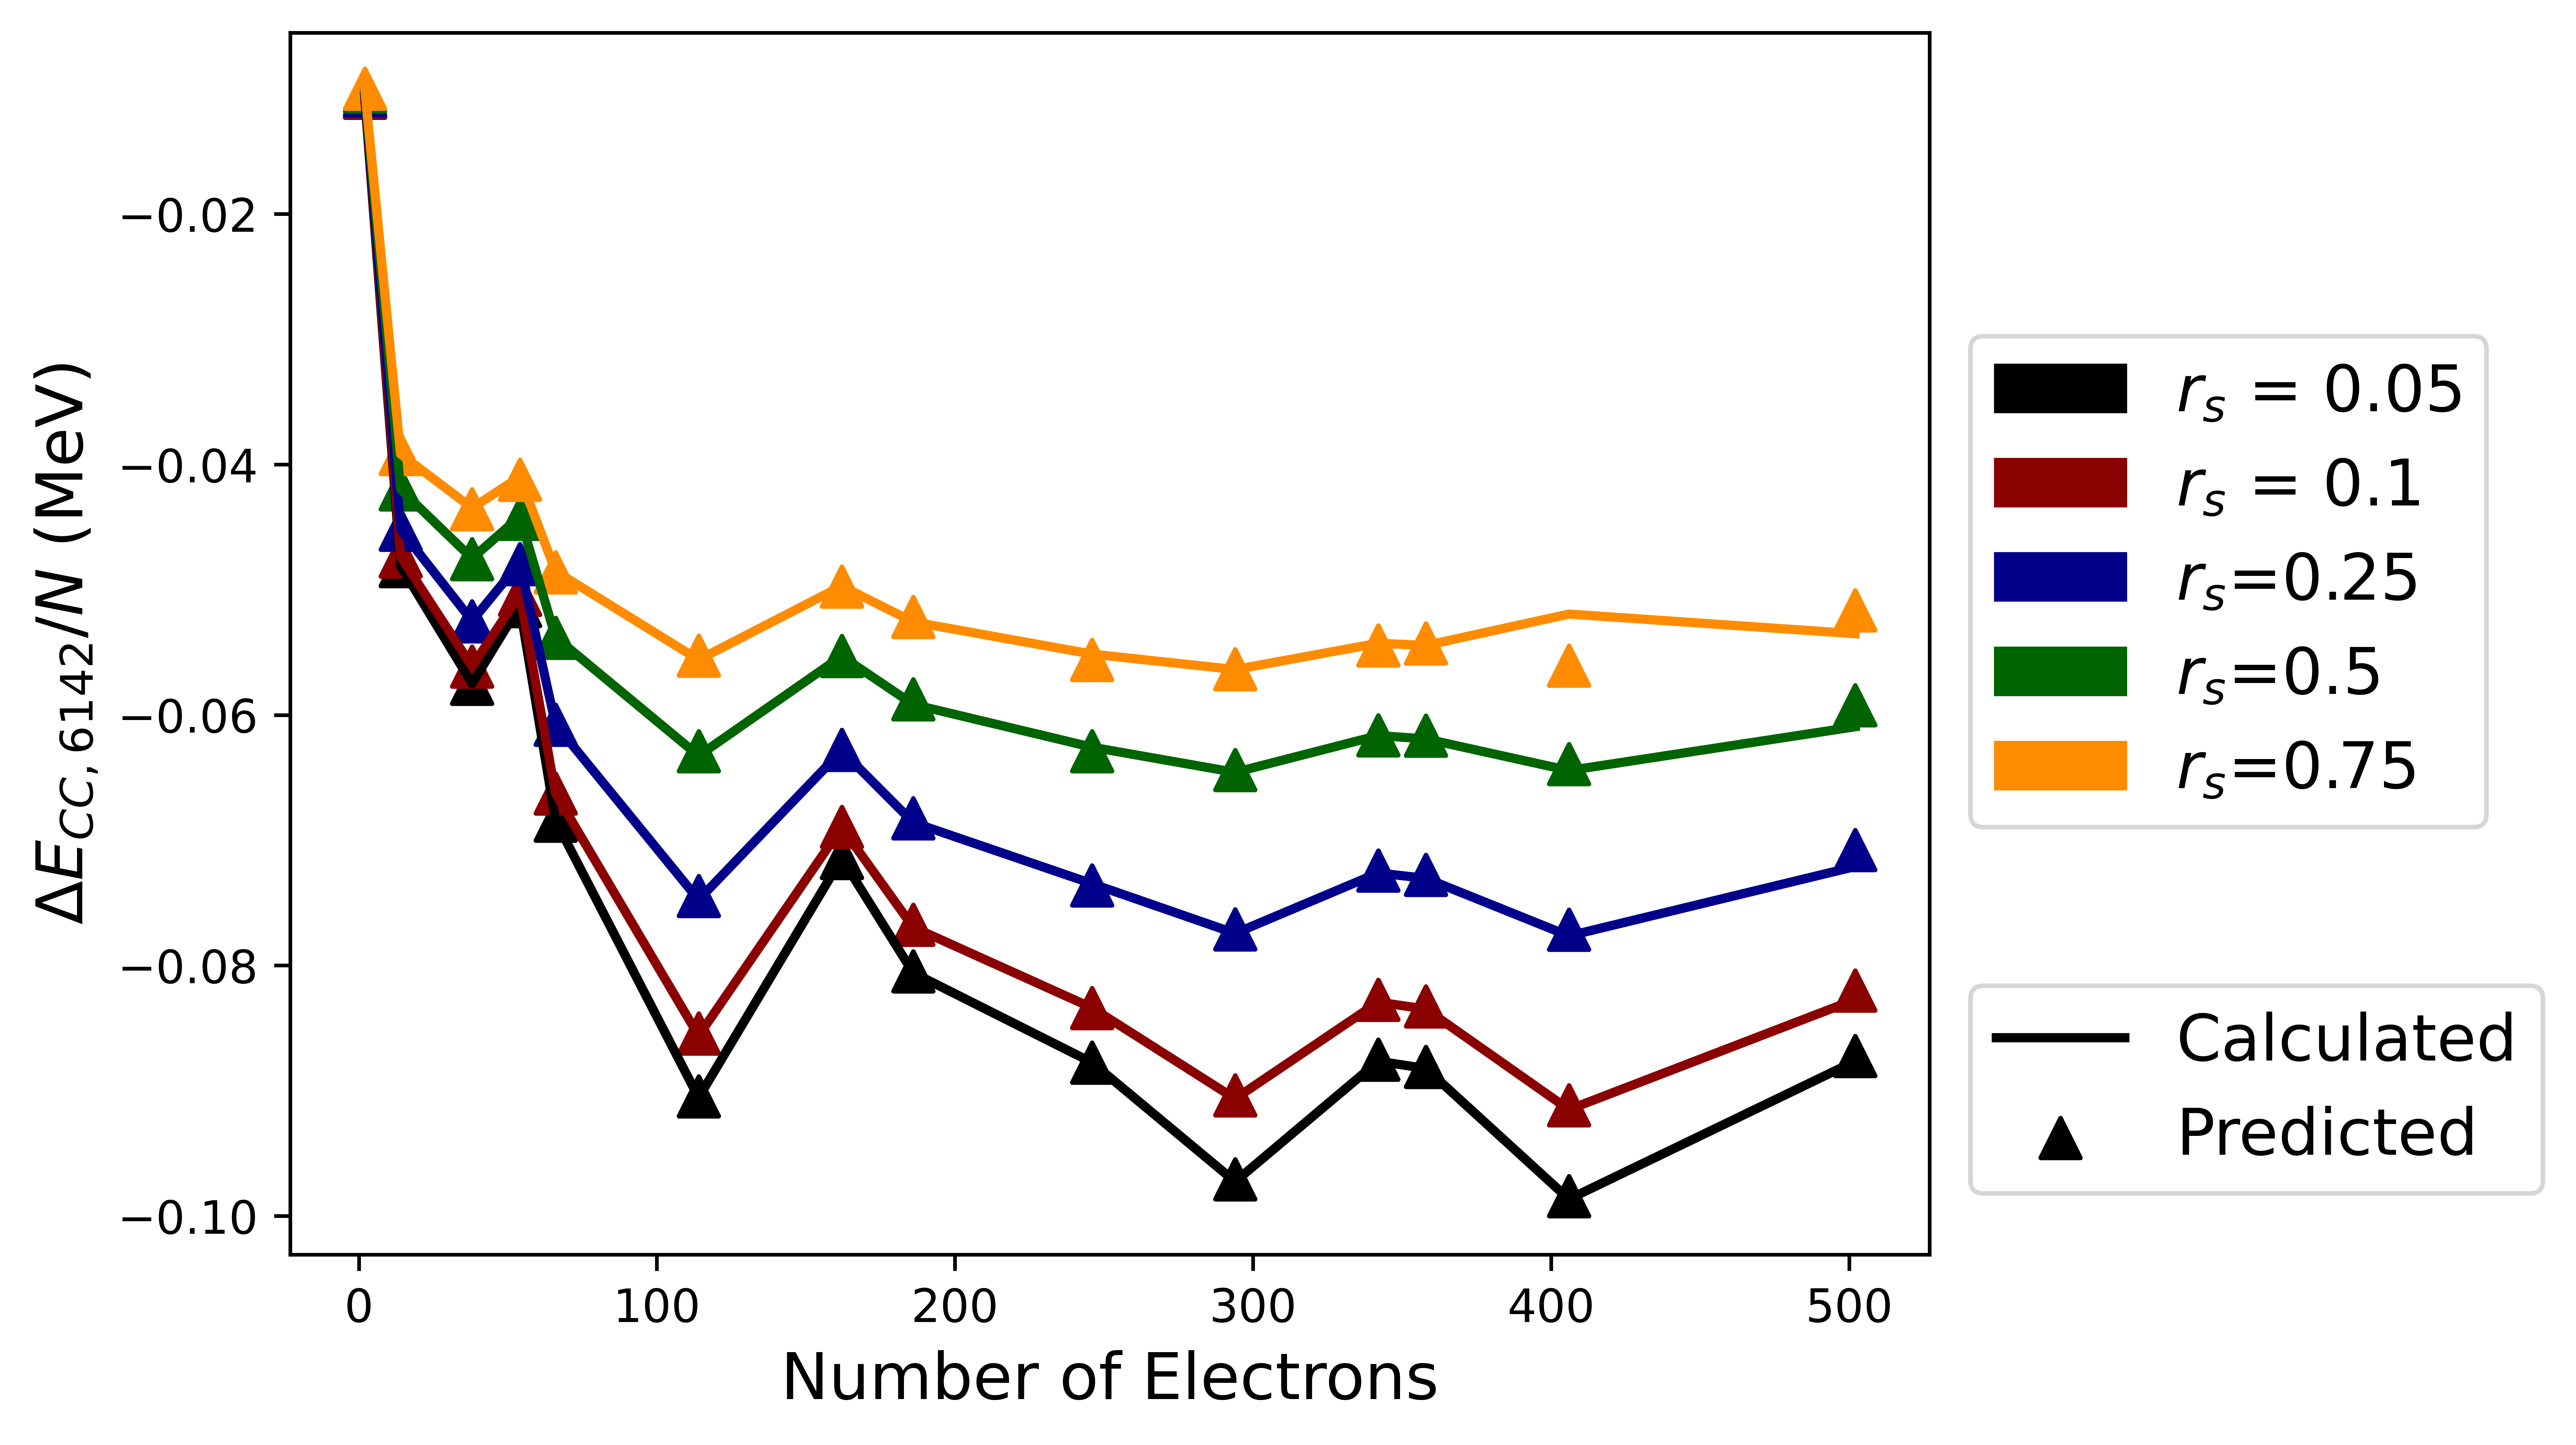
\includegraphics[scale=0.75]{Images/Chapter7/ElectronGas/rs_0_5_EG_Ridge.png}
    \caption{The results of performing an SRE analysis on the HEG to predict the converged CCD correlation energies for 14 different numbers of electrons and five different values of $r_s$.  The SRE predictions, made using a ridge regression algorithm with $\alpha$ = 1x10$^{-10}$, are shown with the triangular markers and the solid lines representing the full correlation energy calculations at M = 6,142. The average percent error between the SRE predictions and the full calculations is 0.45$\%$.}
    \label{fig:rr_tune}
\end{figure}

%% explain rr_tune figure
% 6.88978626138889 10.658995645555557
% 38.32024664305556 54.86648150916667

Fig. \ref{fig:rr_tune} shows the results of performing an SRE analysis on the HEG data set using a ridge regression algorithm with $\alpha$ = 1x10$^{-10}$. This value was chosen because it produces the smallest validation error when performing hyperparameter tuning with the $r_s$ = 0.5 data set. The SRE training procedure was the same as described earlier in this section. The average percent error across all data points in Fig. \ref{fig:rr_tune} is 0.45$\%$, which is tiny. This error is an acceptable level of accuracy of the machine learning predictions, especially considering the potential computational time and resource savings. 

The time needed to generate the training data for the hyperparameter tuning process (i.e., the correlation energies from 5 to 20 open shells for $r_s$ = 0.5) was 6.88 hours. However, the time needed to generate the validation data set (i.e., the correlation energies at M = 6,142 for $r_s$ = 0.5) was 10.65 hours, meaning that the total time needed to generate the data needed for the hyperparameter tuning was 17.53 hours sp there is considerable time to find the optimal value of $\alpha$. If we consider performing the SRE analysis on all five HEG data sets, the time needed to generate all training data is 38.32 hours. Compared to the time needed to generate all $\Delta E_{CC,6142}$ at 54.86 hours, this leads to a time savings for the SRE method of 16.54 hours, or over half a day of computational time saved using the SRE method over doing the complete calculations with no loss of relevant accuracy as the average percent error is less than 0.5$\%$. However, when we add the time needed to generate the validation data set to tune $\alpha$, the time savings drops to only 5.89 hours, which is a much less attractive savings.

%% computational resources discussion

%% Explain the motivation for Bayesian algorithms
Though the SRE algorithm with ridge regression can accurately recreate the converged $\Delta E_{CC}$ for the electron gas at various high densities, the results also display a significant dependence on the hyperparameter $\alpha$ value. Because of this dependence, the fully calculated converged $\Delta E_{CC}$ are not also available, as they are in this work; for comparison, it could be easy to choose a value of $\alpha$ which created a set of converged $\Delta E_{CC}$ which visually look feasible but are not accurate (see Fig. \ref{fig:vary_alpha} for examples). Furthermore, the high computational time and resource requirements needed to generate the validation data set for the hyperparameter tuning process are unattractive. Therefore, we wish to develop a method that can provide the accuracy displayed in Fig. \ref{fig:rr_tune} without dependence and reliance on hyperparameters. Thus, we will start to investigate the Bayesian machine learning implementation of ridge regression: Bayesian ridge regression.
